%\documentclass{acm_proc_article-sp}
%\usepackage{hyperref}
\documentclass{sigplanconf}
%\documentclass[preprint]{sigplanconf}
\usepackage{graphicx}
\usepackage{listings}
\usepackage{epsfig}
\usepackage[all]{xy}

\newcommand{\cL}{{\cal L}}

\begin{document}
\lstset{language=Haskell, numbers=left,
numberstyle=\tiny,numbersep=5pt,basicstyle=\scriptsize,aboveskip=20pt}


\conferenceinfo{GPCE �08}{October 19--23, 2008, Nashville, Tennessee, USA.}
\copyrightyear{2008}
%\copyrightdata{1-59593-056-6/05/0008}

\title{Scenario Variability as Crosscutting}

\authorinfo{Rodrigo Bonif\'{a}cio \and Paulo Borba}
{Informatics Center \\ Federal University of Pernambuco}
{\{rba2,phmb\}@cin.ufpe.br}


\maketitle              

\begin{abstract}
Variability management is a common challenge for Software Product
Line (SPL) adoption, since developers need suitable
mechanisms for describing or implementing variability
that might occur at different SPL views (requirements, design,
implementation, and test). In this paper, we present an approach for
use case scenario variability management, enabling a better
separation of concerns between languages used to manage
variabilities and languages used to specify use case scenarios. The
result is that both representations can be understood and evolved in
a separated way. We achieve such a goal by modeling variability management
as a crosscutting phenomenon, for the reason that artifacts such as feature models, 
product configurations, and configuration knowledge crosscut each 
other with respect to a SPL specific member. Additionally, we argue 
that our proposed approach might be customized to describe variability
mechanisms in other SPL artifacts, being a contribution for
automatic product generation and traceability.
\end{abstract}

\category{D.2.1}{Software Engineering}{Requirements}[Languages,
Methodologies]\
\category{D.2.13}{Software Engineering}{Reusable
Software}

\terms{Design, Documentation}

\keywords{Software product line, variability management, requirement models}

%
\section{Introduction}
%
Software Product Line (SPL) development is a well known technique for 
improving systematic reuse by considering the common features of products in a 
shared domain~\cite{northrop-spl-book}. From a technical point of view, 
SPL approach aims at customizing products from a set of reusable assets. 
In order to do that, developers must represent variation points in the SPL 
assets and describe composition rules which guide product derivation based 
on a specific feature selection~\cite{phol-spl-book}. 

However, \emph{variability management} concern, due to its inherent crosscutting
nature, is a common challenge in product line
adoption~\cite{northrop-spl-book,phol-spl-book}. Such a crosscutting
characteristic is materialized whenever a feature requires variation points to be
spread in different SPL artifacts. Actually, the representation of a variant
feature is often spread not only in several artifacts, but also at the different
product line views (requirements, design, implementation, and test).
Consequently, variability management, in the same way as the feature model and
the architecture, represents a central concern in SPL development and should not
be tangled with existing artifacts~\cite{phol-spl-book}.
 Several authors have proposed the use of \emph{aspect-oriented} mechanisms in
 order to better modularize the composition of common and variant assets of a
 product line~\cite{sousa:aosd-ea04, moreira-re07, eriksson-splc-2005,
 alves-gpce-06, apel-icse2006}.
However, in this paper we go beyond this composition issue. We mainly consider a
more encompassing notion of variability management, including artifacts such as
feature models~\cite{gheyi-alloy-06,czarnecki-book} and configuration
knowledge~\cite{czarnecki-book, phol-spl-book}, and explain it  as a crosscutting
phenomenon.

In this paper, we apply this view of \emph{variability management as
crosscutting} for modularizing SPL use case scenarios. The choice of applying our
approach in this context was motivated because current techniques for scenario
variability
management~\cite{favaro-icsr-98,bertolino-esec-2003,eriksson-splc-2005} do not
present a clear separation between variability management and scenario
specification. As consequence, supposing that details about product variants are
tangled with  use case scenarios, if one variant is removed from the product
line, it would be necessary to change all related scenarios. In summary, when
variability management is tangled with requirements, the evolution of a SPL is
compromised, being difficult to introduce new product variants. The same is true
when this kind of tangling occurs with other software assets, such as design,
source code, and test artifacts.

Another problem is the lack of a formal representation for deriving product
specific scenarios, which is not suitable for current SPL generative
practices~\cite{krueger-cacm-200712}; following the aforementioned works, it is
difficult to automatically derive the requirements of a specific SPL member and
to check if the specified compositions between common and variant scenarios are
correct.  Although  the semantic composition of PLUC (Product Line Use
Case)~\cite{bertolino-esec-2003} is defined in~\cite{fantechi-splc-2004}, such an
approach does not separate scenario specification from variability management, as
presented in Section~\ref{sec:example}.

In order to describe our approach, we propose 
a framework for modeling the composition processes of scenario variabilities with feature models, product configuration, and configuration knowledge (Section~\ref{sec:models}). 
Such a framework aims to: (1) represent a clear separation between variability management 
and scenario specification; and (2) specify how to weave these representations in order to generate
specific scenarios for a SPL member. Therefore, the main contributions of this work are

\begin{itemize}

\item Characterize the broader notation of variability management as a crosscutting concern and, in this way, propose an approach for representing it as an independent view of the SPL. Although this work focuses on requirements artifacts, 
more specifically use case scenarios, we argue that such separation is also valid for other SPL views. Actually,
it has already been claimed for source code~\cite{alves-gpce-06, apel-icse2006}, without considering the importance of variability artifacts.  
  
\item A framework for modeling the composition processes of scenario variability mechanisms. 
This framework gives a basis for describing variability mechanisms (such as scenario composition and parameterization), 
allowing a better understanding of each of them. In this work, such a framework is used for modeling 
the semantics of scenario variability mechanisms, but it might be customized for other SPL views.

\item Describe three scenario variability mechanisms (selection of optional scenarios, scenario composition, scenario parameterization) 
using the modeling framework. Such descriptions present
a more formal representation when compared to existing works; this is an
important property for supporting the automatic derivation of product
specific artifacts.

\end{itemize}

Since our concept of crosscutting mechanism is based on Masuhara and Kiczales work~\cite{kiczales-ecoop-2003}, another 
contribution of this paper is that we apply their ideas to the languages of variability management,  reinforcing the generality of their model, which was originally instantiated only for mechanisms of aspect-oriented programming languages. Based on their view of crosscutting, we can reason about variability management as a crosscutting concern, since different input specifications contribute to derive a specific SPL member. 

Finally, we evaluate our approach (Section~\ref{sec:evaluation}) by comparing it 
to existing works on different product lines.  We 
also relate our work with other research topics (Section~\ref{sec:related}) and present 
our concluding remarks in Section~\ref{sec:conclusions}.

%-----------------------------------------------------------------------
% Subsection: Motivating example
%-----------------------------------------------------------------------
\section{Motivating Example}
\label{sec:example}

In order to customize specific products, by selecting a valid feature
configuration, variantion points must be represented in the product line
artifacts. Several variant notations have been proposed for use case scenarios,
like  Product Line Use Cases (PLUC)~\cite{bertolino-esec-2003} and Product Line
Use Case Modeling for Systems and Software Engineering
(PLUSS)~\cite{eriksson-splc-2005}. However, besides the benefits of variability
support, existing works do not present a clear separation between variability
management and scenario specifications. In this section we illustrate the
resulting problems using the \emph{eShop Product Line}~\cite{eshop-url} as a
motivating example.

The main use cases of the \emph{eShop Product Line} (EPL) allow the user to
\emph{Register as a Customer}, \emph{Search for Products}, and \emph{Buy
Products}.  Five variant features are described in the original specification,
allowing a total  of 72 applications to be derived from the product
line~\cite{eshop-url}. Here, we consider extra features, such as \emph{Update
User Preferences}, which, based on the user historical data of searches and
purchases, updates user preferences. Figure~\ref{fig:eshop-fm} presents part of
the \emph{eShop} feature model~\cite{gheyi-alloy-06,czarnecki-book}; the
relationships between a parent and its child are categorized as: \emph{Optional}
(features that might not be selected in a specific product), \emph{Mandatory}
(features that must be selected, if the parent is also selected), \emph{Or} (one
or more subfeatures might be selected), and \emph{Alternative} (exactly one
subfeature must be selected for each product).

 \begin{figure}[h]
 \begin{center}
  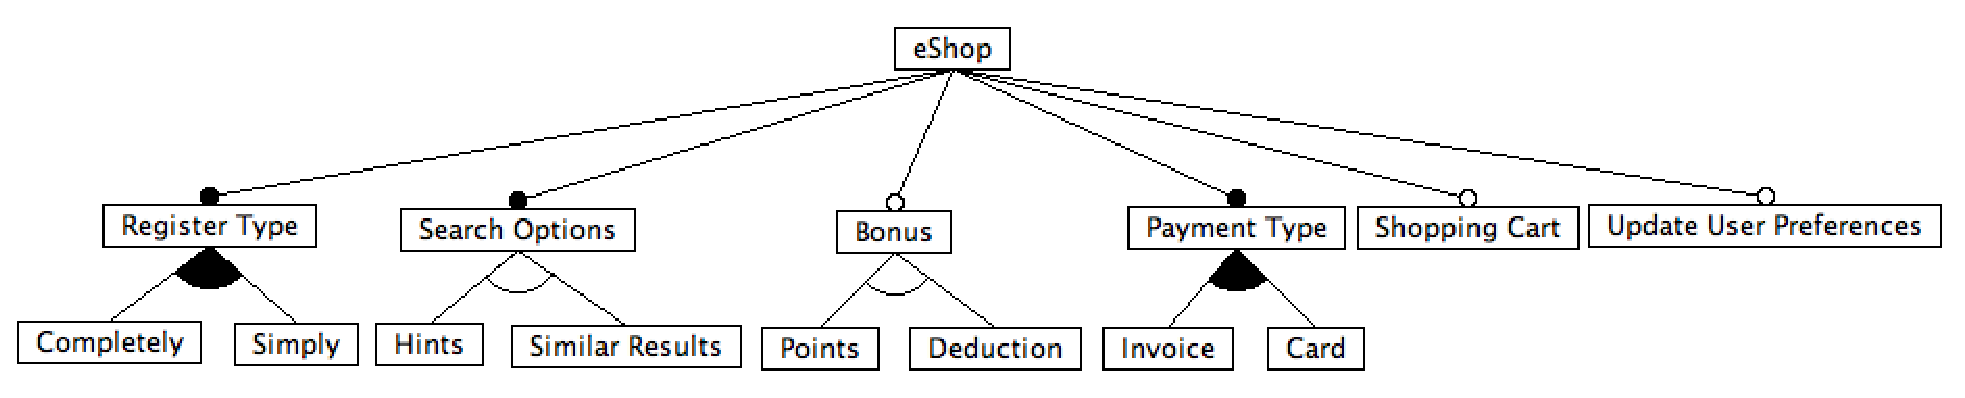
\includegraphics[scale=0.25]{img/eShop-fm3.eps}
   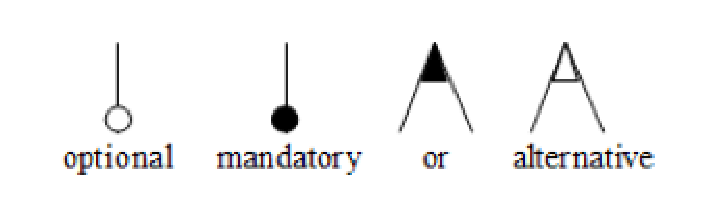
\includegraphics[scale=0.30]{img/fm-notation.eps}
  \nocaptionrule \caption{eShop feature model.}
  \label{fig:eshop-fm}
  \end{center}
\end{figure}



%Other approaches are based on use case extensions~\cite{jacobson-reuse-book}, not explored here since they 
%require that one use case extension must be defined for each variant. This can result in a huge
%number of use cases that is not suitable for managing activities.

In the PLUSS approach, all variant steps of a scenario specification are defined
in the same artifact. For example, steps 1(a) and 1(b) in Figure
~\ref{fig:pluss-01} are never performed together. They are alternative steps:
Step 1(a) will be present only if the \emph{Shopping Cart} feature is selected
(otherwise Step 1(b) will be present)\footnote{Due to space constraints, we
do not represent the relationships between features and PLUSS scenarios in this
paper.}. In a similar way, we have to choose between options (a) and (b) for
Step 2 (depending on the \emph{Bonus Feature} has been selected or not). Finally, Step 6 is optional and will be present only if the feature \emph{Update User Preference} is selected. In this technique, such
restrictions are documented in feature models.

Following this approach, it is hard to understand the behavior of a specific
product because all possible variants are described in the same artifact.
Therefore, it is not possible to reason about scenarios in a modular way.
Moreover, such tangling between variant representation and scenario
specification results in maintainability issues: introducing a new product variant might require changes in several points of existing artifacts.  For example, including a
\emph{B2B Integration} feature, which allows the integration between partners in
order to share their warehouses, might change the specification of the \emph{Buy
Product} scenario, enabling the search for product availability in remote
warehouses (a new variant for Step 1) and updating a remote warehouse when the
user confirms the purchase (a new variant for Step 5). Moreover, the inclusion of
this new optional feature also changes the specification of the \emph{Search for
Products} scenario (the search might also be remote). In summary, since the
behavior of certain features may be spread among several specifications and each
specification might describe several variants, the effort needed to understand
and evolve the product line might increase.

\begin{figure}[h]
\begin{center}
\begin{scriptsize}
  \texttt{
  \begin{tabular}{|p{0.2in}|p{1.3in}|p{1.3in}|}
   \hline
	Id    & User Action & System Response \\ \hline \hline    
       1(a) &Select the checkout option. & Present the items in the shopping cart and the amount to be paid. The user can remove items from shopping cart. \\  \hline
       1(b) & Select the buy product option. & Present the selected product. The user can change the quantity of item that he wants to buy. Calculate and show the amount to be paid. \\  \hline
       2(a) & Select the confirm option. & Request bonus and payment information. \\  \hline
       2(b) & Select the confirm option. & Request payment information. \\  \hline
       3     & Fill in the requested information and select the proceed option. & Request the shipping method and address.\\  \hline
       4     & Select the \$ShipMethod\$, fill in the destination address and select the proceed option. & Calculate the shipping costs. \\  \hline
       5     & Confirm the purchase. & Execute the order and send a request to the Delivery System in order to dispatch the products. \\  \hline
       6     & Select the close section option. & Register the user preferences.\\  \hline
  \end{tabular}
  } 
\end{scriptsize}
\nocaptionrule \caption{Buy Products scenarios using the PLUSS notation.}
\label{fig:pluss-01}
\end{center}
\end{figure}

Instead of relating each variant step to a feature, PLUC introduces special tags
for representing variabilities in use case scenarios. For example, the VP1 tag in
Figure~\ref{fig:pluc-01}, which also describes the \emph{Buy Products} scenario,
denotes a variation point that might assume the values ``\emph{checkout}'' or
``\emph{buy item}'', depending on which product is configured. For each
\emph{alternative} or \emph{optional} step, one tag must be defined. The actual
value of each tag is specified in the \emph{Variation Points} section of the
scenario specification.

\begin{figure}[h]
\begin{center}
\begin{scriptsize}
  \texttt{
  \begin{tabular}{{|p{0.05in}p{3in}|}}
  \hline
  & {\bf Buy Products Scenario} \\
  & {\bf Main Flow} \\
  01 & Select [VP1] option \\
  02 & [VP2] \\
  03 & Select the confirm option \\
  04 & [VP3] \\
  05 & Fill in the requested information and select the proceed option \\
  06 & Request the shipping method and address \\
  07 & Select the [VP4] shipping method, fill in the destination address and select the proceed option \\
  08 & Calculate the shipping costs. \\ 
  09 & Confirm the purchase. \\
  10 & Execute the order and sends a request to the Delivery System in order to dispatch the products \\  
  11 & Select the close section option. \\ 
  12 & \{[VP5] Register the user preferences.\} \\  & \\
  & {\bf Products definition: } \\ & VP0 = (P1, P2) \\ & \\
  & {\bf Variation points: } \\ 
  &  VP1 =  if (VP0 == P1) then (checkout) \\ & \hspace{0.25in} else (buy product) \\
  & VP2 =  if (VP0 == P1) \\ & \hspace{0.25in}  then (Presents the items in the shopping cart...) \\ & \hspace{0.25in} else (Present the selected product. The user...) \\
  & VP3 =  if (VP0 == P1) \\ & \hspace{0.25in} then ( Requests bonus and payment information.) \\ & \hspace{0.25in} else (Requests payment information.) \\
  & VP4 =  (Economic, Fast) \\
  & VP5 requires (VP0 == P1) \\ \hline
   \end{tabular}
  } 
\end{scriptsize}
\end{center}
\nocaptionrule \caption{Buy Products scenarios using the PLUC notation.}
\label{fig:pluc-01}

\end{figure}

A different kind of tangling occurs in this case, since segments of the
specification are tangled with the variation points. Additionally, SPL members
are also described using the same tag notation (see the \emph{Product Definition}
section in Figure~\ref{fig:pluc-01}). There is no explicit relationship between
product configurations and feature models. In the example, two products (P1 and
P2) are defined. The first product is implicitly configured by selecting the
\emph{Shopping Cart}, \emph{Bonus}, and \emph{Update User Preferences} features.
The second model, on the other hand, is not configured with such features.

Since the values of alternative and optional variation points are computed based
on the defined products, instead of specific features, the inclusion of a new
member in the product line might require a deep review of variation points.
Moreover, since the variation points and the product definitions are spread among
several scenario specifications, it is hard and time consuming to keep the SPL
consistent. Finally, the same definitions (product configuration and variation
points) often are useful to manage variabilities in other artifacts, such as
design and source code. As a consequence, this approach requires the replication
of such definitions in different SPL views --- when the SPL evolves, changes are
propagated throughout many artifacts.

In summary, both approaches are not suitable for modularizing the crosscutting
nature of certain features, have poor legibility, and lead to lower
maintainability. Consequently, we argue that the variability
management concern should be separated from the other artifacts and used as a
language for supporting product configuration and traceability. 

% Furthermore,
% in order to support the automatic derivation of product specific artifacts, 
% it is necessary not only to have a more precise definition of each language used
% to describe product line artifacts and the variability management concern, but
% also to formalize the weaving processes used to combine them. Although Eriksson et al. 
% defined the metamodel of PLUSS notation~\cite{eriksson-splc-2005}, they do not
% described which languages and processes are used for relating use case
% scenarios to feature models. Likewise, although Fantechi et al. described the
% formal semantics of PLUC~\cite{fantechi-splc-2004}, this approach does not 
% separate variability management from use case scenarios.

The next section describes our approach that considers scenario variability as a
composition of different artifacts. Although in this paper we focus on use case
scenarios, the idea of separating product line artifacts from variability
management (using feature models, product configurations, and configuration
knowledge) is also applied to other SPL views.


%-------------------------------------------------------------------------
% Section: Modeling the Variability Mechanisms
%------------------------------------------------------------------------
\section{Variability as Crosscutting}
\label{sec:models}

Aiming at representing a clear separation between variability management and
scenario specification, and also to describe the weaving processes required to
compose these views, we propose a modeling framework, that slightly generalizes
Masuhara and Kiczales (MK) framework~\cite{kiczales-ecoop-2003}, and instantiate
it for the use case and product line context. The MK framework aims to explain
how different \emph{aspect-oriented} technologies support crosscutting
modularity. Each technology is modeled as a three-part description: the related
weaving processes take two programs as input, which crosscut each other with
respect to the resulting program or computation~\cite{kiczales-ecoop-2003}.

Similarly to the MK framework, we represent the semantics of \textbf{scenario
variability management} as a weaver that takes as input four specifications
(\emph{product line use case model}, \emph{feature model}, \emph{product
configuration}, and \emph{configuration knowledge}) that crosscut each other with
respect to the resulting product specific use case model
(Figure~\ref{fig:weave-process}). Combining these input languages, it is possible
to represent the kinds of variability that we are interested in: \emph{optional
use cases and scenarios}, \emph{quantified changed scenarios}, and
\emph{parameterized} scenarios.

A running example of our approach is presented in Section~\ref{sub:running}.
After that, we describe the semantics of our weaving process. For simplicity, it
was decomposed in three parts --- one weaver process for each kind of
variability.  The semantics of those weavers (and the meta-model of the input and
output languages) are described using the Haskell programming
language~\cite{haskell-report}. This leads to concise weaving process
descriptions (the related source code is available at a web site~\cite{spg-url})
and keeps our model close to MK work, where weaving processes are specified in
the Scheme programming language. 

% The choice for Haskell was motivated by several factors, such as the existence
% of mature verification tools (QuickCheck and HUnit), readability, and our
% previous background in the language.
 
% \begin{figure}[h] 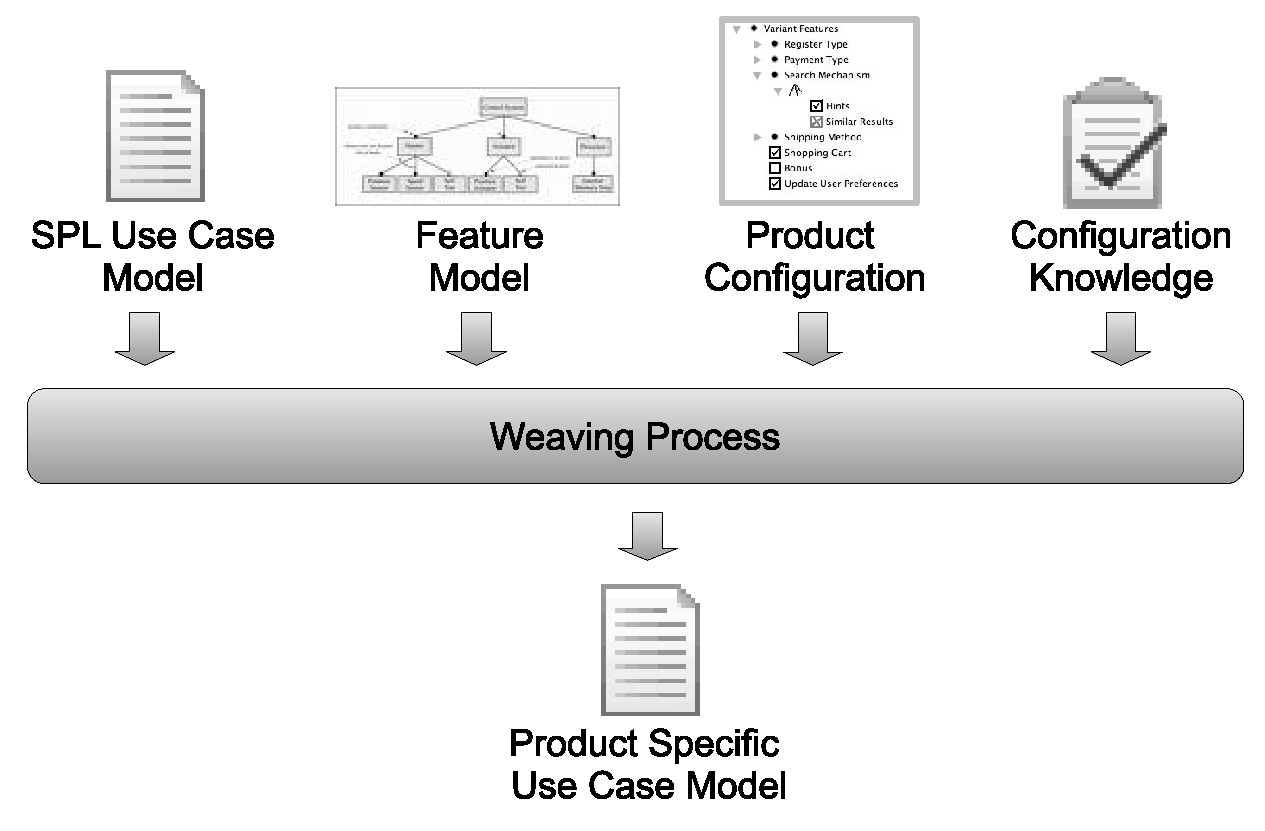
\epsfig{file=img/weave-process2.eps,scale=0.3}
% \caption{Overview of the modeling framework.} \label{fig:weave-process}
% \end{figure}

\begin{figure}[h]
 \begin{center}
  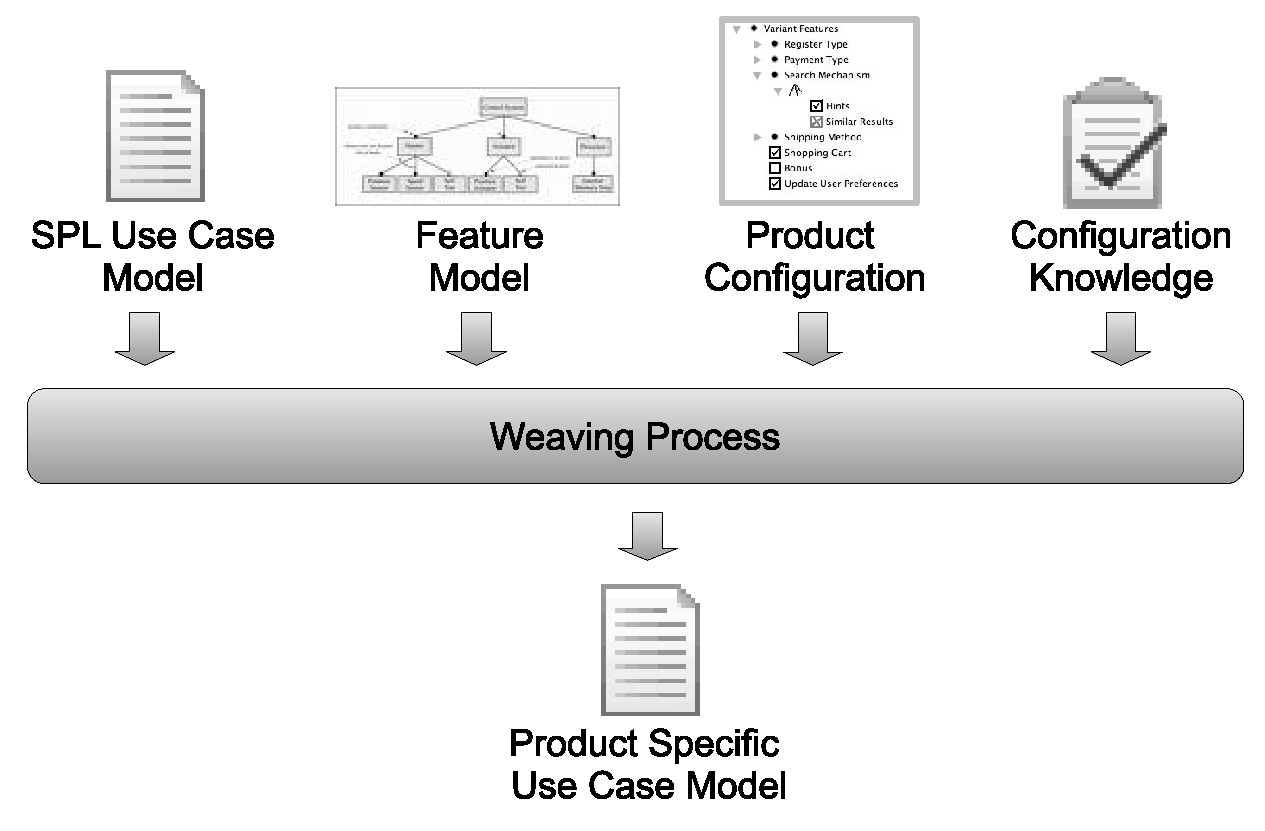
\includegraphics[scale=0.35]{img/weave-process2.eps}
  \nocaptionrule \caption{Overview of our weaving process.}
  \label{fig:weave-process}
  \end{center}
\end{figure}

\subsection{Running Example}
\label{sub:running}

In order to explain how the input languages crosscut each other and produce a
product specific use case model, here we present a running example of our
approach based on the eShop Product Line (briefly introduced in
Section~\ref{sec:example}). For this, several artifacts of each input language
are described. Then, we present the role of each input language in respect of the
weaving process.


\subsubsection{SPL use case model}

This artifact defines a set of scenarios that might be used to describe possible
products of the SPL. Although not being directly concerned with variability
management, some scenarios might be optional, might have parameters, or might
change the behavior of other scenarios. Moreover, a use case scenario corresponds
to a sequence of pairs \emph{User Action} x \emph{System Response}.  A use case
defines a set of scenarios; and a use case model defines a set of use cases. In
this running example, we consider the following scenarios:

{\bf Buy a Product:} this optional scenario
(Figure~\ref{fig:buy-product-scenario}) enables a customer to buy specific goods
from an online shopping store. It is only available at instances of the product
line that are not configured with the \emph{Shopping Cart} and \emph{Bonus}
features. This scenario starts from the IDLE special state  (does not extend the
behavior of an existing scenario) and finishes at the Step P1 of the
\emph{Proceed to Purchase} scenario (which is described later). The clauses
\emph{From step} and \emph{To step} are used for describing the possible starting
and ending points of execution.

\begin{figure}[h]
\begin{scriptsize}
  \texttt{
   \begin{tabular}{l}
     Description: Buy a specific product\\
     From step: IDLE \\
     To step: P1
   \end{tabular}  
  \begin{center} 
  \begin{tabular}{|p{0.1in}|p{1.4in}|p{1.4in}|}
   \hline
       Id    & User Action  & System Response \\ \hline \hline
       B1 & Select the buy product option.  & Present the selected product. The user can change the quantity of items he wants to buy. Calculate and show the amount to be paid. \\  \hline
       B2 & Select the confirm option. &  Request payment information. \\  \hline
    \end{tabular}
  \end{center}
  } 
\end{scriptsize}
\nocaptionrule \caption{Buy product scenario.}
\label{fig:buy-product-scenario}
\end{figure}


{\bf Buy Products with Shopping Cart and Bonus:} this optional scenario
(Figure~\ref{fig:buy-product-changing-flow}) allows the purchasing of products
that have been previously added to a customer shopping cart. It changes the
behavior of the \emph{Buy a Product} scenario by replacing its first two steps
and by introducing the specific behavior required by the \emph{Shopping Cart} and
\emph{Bonus} features. This scenario also starts from the IDLE state (\emph{From
step} clause) and finishes at Step P1 of \emph{Proceed to Purchase} (\emph{To
step} clause). This behavior is required for products that are configured with
\emph{Shopping Cart} and \emph{Bonus} features.

\begin{figure}[h]
\begin{scriptsize}
  \texttt{
   \begin{tabular}{l}
     Description: Buy products using a shopping-cart\\
     From step: IDLE \\
     To step: P1
   \end{tabular}  
  \begin{center} 
   \begin{tabular}{|p{0.1in}|p{1.4in}|p{1.4in}|}
   \hline
       Id & User Action & System Response \\ \hline \hline
       V1 & Select the checkout option.  & Present the items in the shopping cart and the amount to be paid. The user can remove items from the shopping cart. \\  \hline
       V2 & Select the confirm option. & Request bonus and payment information. \\  \hline
  \end{tabular}
  \end{center}
  } 
\end{scriptsize}
\nocaptionrule \caption{Buy products with shopping cart scenario.}
\label{fig:buy-product-changing-flow}
\end{figure}

{\bf Proceed to Purchase:} this mandatory scenario
(Figure~\ref{fig:proceed-to-checkout}) specifies the common behavior that is
required for confirming a purchase. Instances of the product line must be
configured with this scenario. Although it can be started  either after Step B2
(from \emph{Buy a Product} scenario) or after Step V2 (from \emph{Buy Products
with Shopping Cart} scenario), just one of the paths can be available at a
specific product. It is important to notice that the \emph{From step} and
\emph{To step} clauses are used for composing, in a quantified way, different
scenario configurations without specifying all possible variants in a single
artifact (as suggested in the PLUSS notation). Moreover, notice that a parameter
\emph{ShipMethod} is referenced in Step P2 of
Figure~\ref{fig:proceed-to-checkout}. The use of this parameter (notation also
supported in PLUSS and PLUC) allows the reuse of this specification for different
kinds of \emph{ship method} configurations.

\begin{figure}[h]
\begin{scriptsize}
  \texttt{
   \begin{tabular}{l}
     Description: Proceed to purchase\\
     From step: B2, V2 \\
     To step: END
   \end{tabular}  
  \begin{center} 
  \begin{tabular}{|p{0.1in}|p{1.4in}|p{1.4in}|}
   \hline
       Id    & User Action  & System Response \\ \hline \hline
       P1 & Fill in the requested information and select the proceed option.  & Request the shipping method and address.\\  \hline
       P2 & Select one of the available ship methods (\mbox{<ShipMethod>}), fill in the destination address and proceed. & Calculate the shipping costs. \\  \hline
       P3 & Confirm the purchase. & Execute the order and send a request to the Delivery System to dispatch the products. 
       \mbox{[RegisterPreference]} \\  \hline
  \end{tabular}
  \end{center}
  } 
\end{scriptsize}
\nocaptionrule \caption{Proceed to purchase scenario.}
\label{fig:proceed-to-checkout}
\end{figure}

 
{\bf Search for Products:} this mandatory scenario allows the user to search for
products. In order to save space, we are only presenting Step S3, which performs
a search based on the input criteria (Figure~\ref{fig:search-products-flow}).
This step is annotated with the mark \mbox{{\bf [RegisterPreference]}}, exposing
it as a possible extension point for the behavior of \emph{Register User
Preferences}. The same annotation was used in the Step P3 of \emph{Proceed to
Purchase} (Figure~\ref{fig:proceed-to-checkout}). Such annotations can be
referenced in the \emph{from step} and \emph{to step} clauses, reducing problems
that might occur by changing step ids.

\begin{figure}[ht]
\begin{scriptsize}
  \texttt{
   \begin{tabular}{l}
     Description: Search for Products scenario\\
     From step: IDLE \\
     To step: END
   \end{tabular}  
  \begin{center} 
   \begin{tabular}{|p{0.1in}|p{1.4in}|p{1.4in}|}
   \hline
       Id & User Action &  System Response \\ \hline \hline
       \ldots & \ldots  & \ldots \\  \hline
       S3 & Inform the search criteria. &  Retrieve the products that satisfy the search criteria. Show a list with the resulting products. [RegisterPreference] \\  \hline
  \end{tabular}
  \end{center}
  } 
\end{scriptsize}
\nocaptionrule \caption{Search for products scenario.}
\label{fig:search-products-flow}
\end{figure}

{\bf Register User Preferences:} this optional scenario updates the user
preferences based on the buy and search products use cases. Its behavior can be
started at each step that is marked with the {\bf [RegisterPreference]} (see the
\emph{from step} clause) annotation and is available in products that are
configured with the \emph{Update User Preferences} feature.

\begin{figure}[h]
\begin{scriptsize}
  \texttt{
   \begin{tabular}{l}
     Description: Register user preferences.\\
     From step: [RegisterPreference] \\
     To step: END
   \end{tabular}  
  \begin{center} 
   \begin{tabular}{|p{0.1in}|p{1.4in}|p{1.4in}|}
   \hline
       Id & User Action &  System Response \\ \hline \hline
       R1 & - &  Update the preferences based on the search results or purchased items. \\  \hline
  \end{tabular}
  \end{center}
  } 
\end{scriptsize}
\nocaptionrule \caption{Register user preferences.}
\label{fig:register-preferences-flow}
\end{figure}

In this running example, we described several scenarios as being optional or
mandatory. It is important to observe that, in our approach, this kind of
information is not specified in scenario documents. Actually, it is necessary to
consider the relationships between scenarios and features in order to realize
which configurations require a specific scenario. As we said at the beginning of
this section, each artifact (feature model, product configuration, configuration
knowledge, and use case model) provides a specific contribution to the definition
of a SPL member.

\subsubsection{Feature model}

We have introduced part of this artifact for the eShop product line in Section~\ref{sec:example}. However, here we 
present only the features required  (Figure~\ref{fig:eshop-fm-re}) for understanding the running example. 

 \begin{figure}[h]
 \begin{center}
  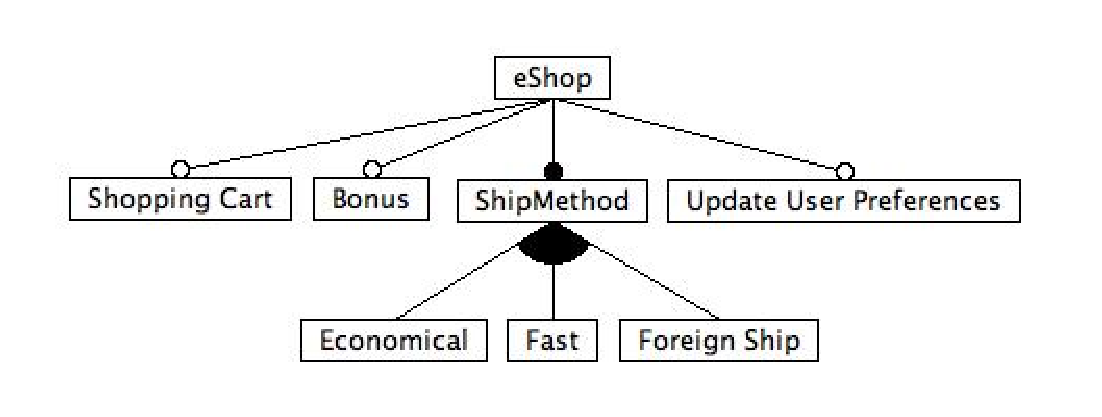
\includegraphics[scale=0.40]{img/eShop-fm-re.eps}
   \nocaptionrule \caption{Subset of eShop feature model.}
  \label{fig:eshop-fm-re}
  \end{center}
\end{figure}

Based on the feature model of Figure~\ref{fig:eshop-fm-re}, the \emph{Shopping 
Cart}, \emph{Bonus} and \emph{Update User Preferences} features are not required; on the other hand, the \emph{Ship Method} feature is mandatory and all products have to be configured with at least one of its child. A short review about the feature model 
notation was presented in Section~\ref{sec:example}. More details can be found elsewhere~\cite{gheyi-alloy-06,czarnecki-book}.  

\subsubsection{Product configuration}

This artifact is used for identifying which features were selected in order to compose a specific member of a product line. Each product configuration should conform to a feature model (the selected features should obey the feature model relationships and constraints). Two possible configurations are presented in Figure~\ref{fig:product-config-01-02}. We represent these configurations as a tree, highlighting which features were selected. Such a representation was created using the \emph{Feature Modeling Plugin}~\cite{czarnecki-eclipse-2004} 

\begin{figure}[htb]
  \centerline{
    \mbox{
\includegraphics[scale=0.4]{img/pc-01.eps}}
    \mbox{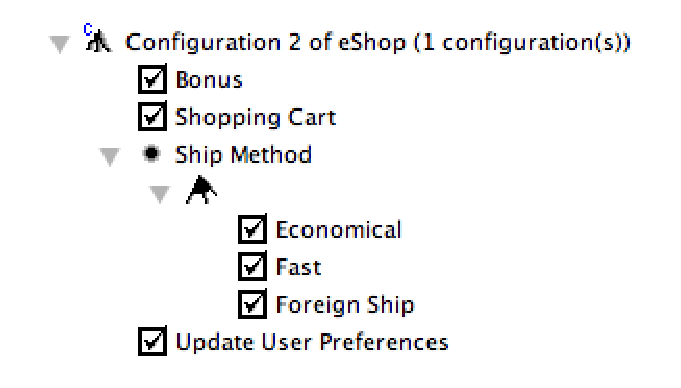
\includegraphics[scale=0.4]{img/pc-02.eps}}
  }
  \nocaptionrule \caption{Examples of product configurations.}
  \label{fig:product-config-01-02}
  \end{figure}
  
The first configuration (on the left side of the Figure~\ref{fig:product-config-01-02}) defines a product that has no support for shopping cart, bonus and preferences update. Additionally, it supports only the economical and fast ship methods. The second configuration selects all possible features. 
In order to select the required assets (scenarios, classes and aspects, test cases) for a specific product configuration, it is necessary to relate features to them. This is the role of the configuration knowledge as an input artifact of our weaving process.  

\subsubsection{Configuration knowledge}

This artifact is used for relating feature expressions to assets that must be assembled in a given product. Such artifacts allow, during product engineering, the automatic selection of assets that are required for a specific product configuration. 

Table~\ref{tab:ck-running-example} presents a configuration knowledge 
for the running example, enforcing that the \emph{Proceed to Purchase} and 
\emph{Search for Products} are mandatory scenarios, since they are related 
to the root feature of eShop product line;  
the \emph{Buy a Product} scenario is used in the composition of products that have not been configured with both \emph{Shopping Cart} and \emph{Bonus} features --- if both features were selected for a product, it will be configured with the \emph{Buy Product with Cart} scenario; and finally, Table~\ref{tab:ck-running-example} states that \emph{Register User Preference} scenario is not used in composition unless the \emph{Update Preference feature} is selected.


\begin{table}[th]
\begin{center}
\nocaptionrule \caption{eShop configuration knowledge}
\label{tab:ck-running-example}
\begin{tabular}{ll}
   \hline\noalign{\smallskip}
  {\bf Expression} & {\bf Required Artifacts} \\
   \noalign{\smallskip}
   \hline
   \noalign{\smallskip}
    eShop & Proceed to Purchase \\
               & Search for Products \\
               & \ldots \\ 
    {\bf not} (Cart {\bf and} Bonus)\hspace{2pt} & Buy a Product \\ 
    Cart {\bf and} Bonus & Buy Products with Cart \\ 
    Update Preferences & Register user Preferences	 \\  
    \ldots & \ldots \\ 
  \hline
\end{tabular}
\end{center}
\end{table}

In what follows, we describe a high level view of the weaving process that combines the input languages in order to manage scenario variability.  Then, in Section~\ref{sub:modeling-framework} we formally present its semantics in terms of our modeling framework. 

\subsubsection{Weaving process}

The weaving process represented in Figure~\ref{fig:weave-process} is responsible for performing the following activities: 

{\bf Validation activity:} This activity is responsible for checking if a product configuration is a valid instance of the feature model. If the product configuration is 
valid (it conforms to the relationship cardinalities and constraints of the feature model), the process might proceed. 

{\bf Product derivation activity:} This activity takes as input a (valid) product configuration and a configuration knowledge. 
Each feature expression of the configuration knowledge is checked against the product configuration. If the expression 
is satisfied, the related scenarios are assembled as the result of this activity. For the running example, 
Table~\ref{tab:assembled-scenarios} shows the assembled scenarios for the configurations depicted in Figure~\ref{fig:product-config-01-02}.

\begin{table}[h]
\begin{center}
\nocaptionrule \caption{Assembled scenarios} \label{tab:assembled-scenarios}
\begin{tabular}{ll}
   \hline\noalign{\smallskip}
  {\bf Configuration} & {\bf Assembled scenarios} \\
   \noalign{\smallskip}
   \hline
   \noalign{\smallskip}
    Configuration 1\hspace{15pt} & Proceed to Purchase \\
                                                   & Search for Products \\
                                                   & Buy a Product \\
                             			  & \ldots \\
   Configuration 2                        & Proceed to Purchase \\
                             			  & Search for Products	 \\
			                           & Buy Products with Cart \\
                                                   & Register User Preferences \\
                             & \ldots       \\
  \hline
\end{tabular}
\end{center}
\end{table}
 
 {\bf Scenario composition activity:} This activity is responsible for composing the scenarios assembled for a specific product configuration. 
Therefore, the resulting scenarios of the previous activity, which crosscut each other based on the \emph{From step} and \emph{To step clauses}, are woven. The 
 result is a use case model with complete paths (all \emph{From step} and \emph{To step} clauses are resolved).
 
%  or a trace model (a set of all valid sequences of events extracted from the complete paths). 
 
The complete path is a high level representation, which uses the same constructions of the use case model (scenarios), and is illustrated here as a graph, where each node is labeled with a step id. For example, Figure~\ref{fig:complete-paths} depicts the complete paths for the first and second configurations of our running example. In the left side of the figure,  the composition of \emph{Buy a Product} with \emph{Proceed to Purchase} (branch labeled as B1, B2, P1, P2, P3) and \emph{Search for Product} (branch labeled as S1, S2, S3) scenarios are presented. Contrasting, on the right side of the figure, the results of this activity are presented for the second configuration. In this case, steps B1 and B2 have been replaced by steps V1 and V2 (because \emph{Shopping Cart} and \emph{Bonus} features are selected) and the step  R1 is introduced after steps P3 and S3 (because \emph{Update User Preferences} is selected in this configuration).
 
%=====================
% Trace model discussion
%===================== 
 
%Instead, the trace model can be seen as a low level representation of the use case model. Such notation has a well defined semantic and might 
%be used for model checking and test case generation. Such applications of the trace model are beyond the scope of this paper. More information 
%can be found elsewhere\cite{csp-hoare,csp-roscoe,cfeitosa-sbmf-2006}. Here, the trace model is useful for implementing the last activity of our weave process, binding parameters, and 
%represents all possible sequences of events in a specific product configuration. 

%For instance, the trace model for the first configuration is the set of sequences:

%\begin{small}
%\begin{tabular}{rlc}
%$Trace_{C1}$ = & \{<>, <idle>, <idle, 1S>, <idle, 1S, 2S>, \\ 
%                    & <idle, 1S, 2S, 3S>,  <idle, 1S, 2S, 3S, end>, \\ 
%                    & <idle, 1M>, <idle, 1M, 2M>, \ldots, \\ 
%                    & <idle, 1M, 2M, 3M, 4M.ShipMethod, 5M, end> \}
%\end{tabular}
%\end{small}

%========================
 
\begin{figure}[bth]
\begin{center}
\begin{tiny}
\begin{xy}
\xymatrix@R=10pt{
& *++[o][F-]{idle} \ar[r]\ar[d] & *++[o][F-]{B1} \ar[d]	& *++[o][F-]{idle} \ar[r]\ar[d] & *++[o][F-]{V1} \ar[d] 		\\
& *++[o][F-]{S1} \ar[d]  & *++[o][F-]{B2} \ar[d]           & *++[o][F-]{S1} \ar[d]  & *++[o][F-]{V2} \ar[d] 			\\
& *++[o][F-]{S2} \ar[d]  & *++[o][F-]{P1} \ar[d]           & *++[o][F-]{S2} \ar[d]  & *++[o][F-]{P1} \ar[d]			\\
& *++[o][F-]{S3} \ar[d]  & *++[o][F-]{P2} \ar[d]           & *++[o][F-]{S3} \ar[d]  & *++[o][F-]{P2} \ar[d] 			\\
& *++[o][F-]{end} & *++[o][F-]{P3} \ar[l]                     & *++[o][F-]{R1} \ar[d] & *++[o][F-]{P3} \ar[l]   			\\
&                         &                                                    &   *++[o][F-]{end}       &
}
\end{xy}
\end{tiny}
\nocaptionrule \caption{Complete paths represented  as a graph}
\label{fig:complete-paths}
\end{center}
\end{figure}

{\bf Binding parameters activity:}  This activity weaves scenarios and product configurations in order to resolve all scenario parameters. 
For example, step P2 in Figure~\ref{fig:proceed-to-checkout} has a reference 
 to the \emph{ShipMethod} parameter, whose domain values are defined in the product configuration. For instance, in the first configuration depicted in Figure~\ref{fig:product-config-01-02}, the parameter \emph{ShipMethod} might assume the values \emph{Economical} or \emph{Fast}. 
In order to reduce the coupling between scenario specifications and feature model, a mapping is used for relating scenario parameters to features. In fact, this mapping is another input artifact of our modeling framework; but it was not represented in Figure~\ref{fig:weave-process} because it was just introduced for avoiding explicit dependencies between feature and use case models.  
Next, we introduce the modeling framework used to formally describe the weaving processes just presented. 
%===================
% Trace model discussion
%===================

%For each trace that contains a parameterized event (or step), this activity creates a new trace for all of the possible parameter values. Consequently, resolving parameters for the trace $<idle,1M,2M,3M,4M.ShipMethod>$ results in the following sequences:
% 
%\begin{center} 
%\begin{small}
%\begin{tabular}{c}
%<idle,1M,2M,3M,4M.Economical>, \\ <idle,1M,2M,3M,4M.Fast>, \\
%\end{tabular}
%\end{small}
%\end{center}




\subsection{Modeling Framework}\label{sub:modeling-framework}

As mentioned before, the semantics of crosscutting, used for representing our variability management weaving process, is based on the Masuhara and Kiczales work~\cite{kiczales-ecoop-2003}. 

First of all, their requirement for characterizing a mechanism as crosscutting is fulfilled by our approach, since different specifications contribute to the definition of a specific SPL member. As a consequence, due to its crosscutting nature, the modeling framework proposed in~\cite{kiczales-ecoop-2003}  is suitable for formalizing variability management compositions. 

For simplicity, our weaving process is formally described as being composed by three major weavers: \emph{product derivation weaver}, \emph{scenario composition weaver}, and \emph{bind parameters weaver}. As a customization of MK work, our modeling framework represents each weaver as an 6-tuple (Eq.~\ref{eq:tuple} and Table~\ref{tab:tup-01}), highlighting the contribution of each input language in the composition processes. 

\begin{equation}
W = \{o, o_{jp}, L, L_{id}, L_{eff}, L_{mod}\}, 
\label{eq:tuple}
\end{equation}

\begin{table}[h]
\begin{center}
\nocaptionrule \caption{Modeling framework elements.} \label{tab:tup-01}
\begin{tabular}{|p{0.6in}|p{2.4in}|}
  \hline
  {\bf Element} & {\bf Description} \\ 
   \hline
  $o$              & Output language used for describing the results of the weaving process \\ \hline
  $o_{jp}$       & Set of join points in the output language \\ \hline
  $L$              & Set of languages used for describing the input specifications \\ \hline
  $L_{ID}(l)$      & Set of constructions in each input language $l$, used for identifying the output join points \\ \hline 
  $L_{EFF}(l)$   & For each input language $l$, this element represent the effect of its constructions in the weaving process \\ \hline
  $L_{MOD}(l)$  & Set of modular unities of each input language $l$\\ \hline
  \hline
\end{tabular}
\end{center}
\end{table}

We represent each weaver by 
filling in the six parameters of our 6-tuple representation, and by stating 
how elements of the weaver implementation correspond to elements of the model.

% ---
% Product derivation weaver
% ---
\subsubsection{Product derivation weaver}\label{sub:pd-weaver}

This weaver is responsible for selecting artifacts based on specific product configurations. 
As a consequence, it implements the first two activities of our variability management approach: 
validating a product configuration against  a feature model and selecting a subset of the SPL assets. 
Although in this paper we are focusing only in the selection of scenarios that should be assembled in specific instances 
of the SPL, this weaver can be easily extended for managing variabilities in other kinds of assets (aiming at selecting design elements, source components, and test cases). 

For instance, applying this weaver for combining the eShop use case model, feature model , and configuration knowledge with the configuration depicted in right side of Figure~\ref{fig:product-config-01-02} will result in the selection of  \emph{Buy Products with Cart}, \emph{Proceed to Purchase}, \emph{Search for Products}, and \emph{Register User Preferences} scenarios.  
 This weaver is implemented by the function \emph{pdWeaver} (Listing~\ref{lst:configure}) and takes as input 
a \emph{SPL use case model} (UCM), a \emph{feature model} (FM), a \emph{product configuration} (PC), and a \emph{configuration knowledge} (CK). 

Initially, this function verifies if the product configuration is a well formed instance of the feature model (\emph{validInstance} function) --- if it is not the case,  an \emph{InvalidProduct} error is thrown. Then, the IDs of selected scenarios are computed by the \emph{configure} function. This is done by evaluating which feature expressions, defined in the list elements (x:xs) of configuration knowledge, are valid for the specific product instance (\emph{eval} function). Finally, given the resulting list of scenario IDs, the function \emph{retrieveArtifacts} returns the product specific scenarios. 
As a consequence, we can realize two levels of crosscutting in this weaver. First, the feature model, the product configuration, and the configuration knowledge crosscut each other in order to contribute to the list of valid scenario IDs composition. Then, the resulting list of scenario IDs crosscuts with the use case model for selecting the product specific scenarios.    

\begin{lstlisting}[belowskip=20pt,frame=tb,caption={Product derivation weaver function},label=lst:configure]
pdWeaver :: UCM -> FM -> PC -> CK -> ScenarioList
pdWeaver ucm fm pc ck = 
 if not (validInstance fm pc) 
 then error InvalidProduct
 else retrieveScenarios ucm (configure pc ck)

configure :: PC -> CK -> ListOfScenarioId
configure pc (CK []) = []
configure pc (CK (x:xs)) =
 if (eval pc (expression x))
  then (artifacts x) ++ (configure pc (CK xs))
  else configure pc (CK xs)
\end{lstlisting}

The model of the \emph{Product Derivation Waver}, 
in terms of the framework, is shown in Table~\ref{tab:pd-weaver}. The \emph{pdWeaver} function is used to argue that the model is realizable and appropriate~\cite{kiczales-ecoop-2003}. We achieve this by matching the model elements 
to corresponding parameters and auxiliary functions in the implementation code. Therefore, the input languages UCM, FM, CK, and PC are represented as different parameters 
of the \emph{pdWeaver} function. An instance of the UCM corresponds to the specification of all 
SPL scenarios. A FM instance is only responsible for declaring the SPL features and the relationships between 
them; as a consequence, there is no coupling between FMs and UCMs. Instead, relationships between features and artifacts are documented in the configuration knowledge. Finally, the PC specifies which features were selected 
for a specific product. 

\begin{table}[htb]
\begin{center}
\nocaptionrule \caption{Model of Product Derivation} \label{tab:pd-weaver}
\begin{tabular}{p{0.6in}p{2.4in}}
   \hline\noalign{\smallskip}
  {\bf Element} & {\bf Description} \\
   \noalign{\smallskip}
   \hline
   \noalign{\smallskip}
   $o$               & Product specific scenarios (list of scenarios) \\ 
   $o_{jp}$        & Scenario declarations \\ 
   $L$               & \{UCM, FM, CK, PC\} \\ 
   $UCM_{ID}$ & SPL scenarios \\ 
   $FM_{ID}$    & SPL features \\ 
   $CK_{ID}$    & Feature expressions and scenario IDs\\  
   $PC_{ID}$    & Product specific feature selection \\ 
   $UCM_{EFF}$ & Provides declaration of scenarios \\  
   $FM_{EFF}$    & Checks if a SPL instance is well formed \\ 
   $CK_{EFF}$    & Identifies selected artifacts  \\ 
   $PC_{EFF}$    &Triggers scenario selection \\
   $UCM_{MOD}$ & Scenario \\  
   $FM_{MOD}$   & Feature \\ 
   $CK_{MOD}$    & Each pair $(feature\ expression, artifact\ list)$  \\ 
   $PC_{MOD}$    & Feature \\
  \hline
  \end{tabular}
\end{center}
\end{table}

The UCM has a greater importance over the other input languages ($UCM_{EFF}$), since it declares the parts that compose the product specific scenarios (the 
output of this weaver process generated by the \emph{pdWeaver} function). These scenarios ($UCM_{ID}$) are used in the \emph{retrieveScenarios} function in order to identify which artifacts will be assembled in the final product.     

In order to identify which artifacts are required for a specific product, the \emph{configure} function ($CK_{EFF}$) checks the feature expression ($CK_{ID}$) against the product specific features ($PC_{ID}$). The effect of FM in this weaver ($FM_{EFF}$) is to check if the PC is well formed. Such evaluation is implemented by the \emph{validInstance} function and considers the PC feature selection ($PC_{EFF}$). 
  

% ---
% Scenario composition weaver
% ---

\subsubsection{Scenario composition weaver}\label{sub:sc-weaver}

This weaver is responsible for the third activity of our variability management 
approach. It aims at composing variant scenarios of a use case and is applied whenever a use case scenario supports different execution paths.
This mechanism takes as input the product specific use case model (a list of scenarios). Each scenario, often partially specified, is then composed in order to generate concrete specifications.

As shown in Section{~\ref{sub:running}, a variant scenario 
might refer to steps either in basic or other variant scenarios. In order
to compute the complete paths defined by a scenario, we need to compose the events that precede all steps referenced by its \emph{From step
clause} (up to the IDLE step), followed by its own steps, and then by all
events that follow all of the steps referenced by its \emph{To step clause} (down to the END step). 

For instance, consider a product configured with the features \emph{Shopping Cart} and \emph{Bonus}, which requires the \emph{Buy Products with Cart} scenario, and with the feature \emph{Update User Preferences}. Referring to Figure~\ref{fig:buy-product-changing-flow}, the  \emph{Buy Product with Cart} scenario starts from the IDLE state (\emph{From step} clause) and then, after its own flow of events, goes to Step P1 of \emph{Proceed to Purchase} (see the \emph{To step} clause). In a similar way, Figure~\ref{fig:register-preferences-flow} depicts that \emph{Register User Preferences} scenario starts from any step that is marked with the \emph{RegisterPreferences} annotation (for example, Step P3 of of \emph{Proceed to Purchase}). In this context, the result of applying the composition scenario weaver is a concrete path of execution for this configuration, that can be represented as this sequence of step ids: \mbox{<IDLE, V1, V2, P1, P2.ShipMethod, P3, R1, END>}.

Note that this sequence still has  the \emph{ShipMethod} parameter, 
referred in Step P2 of \emph{Proceed to Purchase} scenario. The \emph{Binding parameter weaver}, discussed in the next section, is responsible for resolving parameters in the final 
product specification.  

%Before formalizing the \emph{Scenario composition weaver}  in terms of our modeling framework, we 
%first discuss about the abstract representation of scenarios (Listing~\ref{lst:ucm}). We omit elements of the use case model abstract syntax that are not required for understanding this weaver. A scenario has an id, a
%description, a \emph{From step clause} (a list of references for
%existing steps), a list of steps, and a \emph{To step clause} (also
%a list of references for existing steps). A step has an id, a
%specification in the form of a tuple
%(user-action x sytem-response), and a list of annotations
%that can be used to semantically identify the step (avoiding
%fragile pointcuts). Finally, a reference to a step can be either a reference to a \emph{step id} or to a \emph{step annotation}.

%\begin{lstlisting}[belowskip=10pt,frame=tb,caption={Abstract syntax of scenario artifact},label=lst:ucm]
%data Scenario = Scenario id FromStep StepList ToStep
%data Step = Step Id Action Response Annotations
%\end{lstlisting}

The \emph{Scenario Composition Weaver} is implemented by the \emph{scWeaver} function (Listing~\ref{lst:trace}), which takes 
as input the product specific use case model (a list of scenarios computed by the previous weaver).  
The \emph{scWeaver} function computes the complete paths of each  
scenario by calling, recursively, the \emph{completePaths} function. This 
function (lines 5-6 in Listing~\ref{lst:trace}) 
takes as input the product specific use case model (\emph{ucm}) and a specific
scenario (\emph{scn});
and returns all complete paths (a list of \emph{step lists}) of
\emph{scn}. The function \emph{fromList} (called at line 7) is used to
compose all complete paths extracted from the \emph{From step
clause}. In a similar way, the function \emph{toList} (called at
line 7) is used to compose all complete paths extracted from the
\emph{To step clause}. The \emph{match} function (also called at
line 7), retrieves all the steps in \emph{ucm} that satisfy all 
\emph{step references} in \emph{From step} or \emph{To step}
clauses. 

%Currently, this matching is based on the \emph{step id} (a
%syntactically reference) or on the list of \emph{step annotations}
%(a semantic reference). The ``+++'' operator denotes distributed
%list concatenation.

\begin{figure*}
\begin{lstlisting}[belowskip=10pt,frame=tb,caption={Scenario composition weaver function},label=lst:trace]
scWeaver :: ScenarioList -> [StepList]
scWeaver scenarioList = [completePaths scenarioList s | s <- scenarioList]
 
completePaths :: ScenarioList -> Scenario -> [StepList]
completePaths ucm scn =
 (fromList ucm (match ucm (fromSteps scn)) +++ [stepsOf scn]) +++  (toList ucm (match ucm (toSteps scn)))

traceModel [] = [[]]
traceModel (x:xs) = [] : (x) ^ (traceModel (xs))
\end{lstlisting}
\end{figure*}

The model of this weaver is in Table~\ref{tab:sc-weaver}. The output ($o$ element of our modeling framework) is the complete paths of the product specific scenarios, computed directly from \emph{scWeaver} function. Therefore, the input language (L) corresponds to the product specific scenarios, related to the \emph{scWeaver} 
 parameters. 
The join points are modeled as the final scenarios and steps in the output language. They result from the composition of partial scenarios by means of 
\emph{from steps} and \emph{to steps} clauses ($L_{ID}$).  
The effect of the input languages ($L_{EFF}$) in the composition process is to combine 
product specific scenarios that, before this activity, did not define a concrete flow of events. As a consequence, the \emph{match} function 
plays a fundamental role in this process, retrieving the steps in the use case model that satisfies the \emph{From step} and \emph{To step} clauses.  

\begin{table}[hbt]
\begin{center}
\nocaptionrule \caption{Model of Scenario Composition Weaver}
\label{tab:sc-weaver}
\begin{tabular}{p{0.4in}p{2.6in}}
   \hline\noalign{\smallskip}
  {\bf Element} & {\bf Description} \\
   \noalign{\smallskip}
   \hline
   \noalign{\smallskip}
   $o$               & List of composed scenarios  \\ 
   $o_{jp}$        & Scenarios and steps of scenarios \\ 
   $L$               & \{Product specific scenarios (list of scenarios)\} \\ 
   $L_{ID}$       & From step and to step clauses \\ 
   $L_{EFF}$    & Defines abstract scenarios  \\ 
   $L_{MOD}$  &  Scenarios \\  
  \hline
  \end{tabular}
\end{center}
\end{table}


After computing the complete paths (using the \emph{scWeaver} function), it is possible to derive another representation for product specific scenarios. This is essentially a \emph{trace model}, since it describe all possible sequences of events specified by the complete paths. This representation is useful for checking, for example, if a non-expected sequence of events is present in a final product, which means that a problem in the composition has occurred. Actually, we used this representation in the verification process of our model (Section~\ref{sub:model-verification}. The \emph{traceModel} function (lines 8 and 9 of Listing~\ref{lst:trace}) is responsible for computing this representation. For instance, the trace model for the the first configuration of our running example is the set of sequences:

\begin{small}
\begin{tabular}{rlc}
$Trace_{C1}$ = & \{<>, <idle>, <idle, S1>, <idle, S1, S2>, \\ 
                    & <idle, S1, S2, S3>,  <idle, S1, S2, S3, end>, \\ 
                    & <idle, B1>, <idle, B1, B2>, \ldots, \\ 
                    & <idle, B1, B2, P1, P2.ShipMethod, P3, end> \}
\end{tabular}
\end{small}


% ---
% Bind parameters weaver
% ---

\subsubsection{Bind parameters weaver}\label{sub:bind-weaver}

This weaver is responsible for the third activity of our variability
management process. Parameters are used in scenario specifications 
in order to create reusable requirements. This kind of variability can be applied
whenever two or more scenarios share the same behavior (the sequence
of actions) and differ in relation only to values of a same concept.
For instance, Figure~\ref{fig:proceed-to-checkout} depicts the \emph{Proceed to Purchase} 
scenario that can be reused for different \emph{ship methods}. Without this
parameterized specification, and aiming, for example, at automatically generating a test case suite 
with a good coverage, it would be necessary to create a specification for each kind of shipment method.

This weaver takes into consideration \emph{scenario specifications} and 
\emph{product configurations}, which defines the domain values of a
parameter. Thus, in order to reduce the coupling between scenarios and features, 
we propose a mapping that relate them. A constraint must be obeyed in this mapping: features related to parameters must be either an {\bf alternative feature} or an {\bf or feature}~\cite{gheyi-alloy-06,czarnecki-wsfactory-2005,czarnecki-book}.

The implementation of this weaver consists of calls to 
the \emph{bpWeaver} function (Listing~\ref{lst:bind}) for each step 
available in the product specific scenarios or complete paths. This
function (lines 1-5 of Listing~\ref{lst:bind}) takes as
input a mapping (\emph{m}), which relates a scenario parameter to a 
feature; a product configuration (\emph{pc}), which defines 
the domain values of parameters (expressed as the feature selection); and a step (\emph{s}) that may be parameterized. Then, it replaces all parameters
from \emph{s}, returning it as a suitable representation with the
corresponding parameter values. Each text between the symbols ``$<$'' and ``$>$''
(defined in the user action or system response of a
step) is treated as a parameter and must be defined in the
mapping.

For example, if a product is configured with either \emph{Economical} and 
\emph{Fast} ship methods, the result of applying this weaver for 
the Step P2 of the \emph{Proceed to Purchase} scenario will result in the 
representation (\emph{Economical or Fast}) in each place that the parameter \emph{ShipMethod} is referred.

Table~\ref{tab:bp-weaver} describes the Bind Parameters model. This weaver just resolves parameters in scenario specifications. Therefore, its output language is also a list of scenarios; but with resolved parameters (the join points). 

\begin{lstlisting}[belowskip=10pt,frame=tb,caption={Bind parameter weaver function},label=lst:bind]
bpWeaver :: Mapping -> PC -> Step -> Step
bpWeaver m pc s =
 if (length (extractParameters (s)) == 0)
  then s
  else replaceParameterValues m pc s
\end{lstlisting}


\begin{table}[th]
\begin{center}
\nocaptionrule \caption{Model of Bind Parameters Weaver} \label{tab:bp-weaver}
\begin{tabular}{p{0.7in}p{2.3in}}
   \hline\noalign{\smallskip}
  {\bf Element} & {\bf Description} \\
   \noalign{\smallskip}
   \hline
   \noalign{\smallskip}
   $o$               & List of scenarios with resolved parameters  \\ 
   $o_{jp}$        & Each resolved parameter \\ 
   $L$               & \{UCM, PC, Mapping\} \\ 
   $UCM_{ID}$ & Parameterized steps \\
   $PC_{ID}$    & Selected features related to parameters \\ 
   $Mapping_{ID}$ & Key entries (parameter name) of the mapping\\
   $UCM_{EFF}$ & Declares parameterized scenarios \\
   $PC_{EFF}$    & Defines the domain value of parameters \\ 
   $Mapping_{EFF}$ & Relates parameters to features \\
   $UCM_{MOD}$ & Use case scenarios \\
   $PC_{MOD}$    & Selected features \\ 
   $Mapping_{EFF}$ & Each entry in the mapping \\
  \hline
  \end{tabular}
\end{center}
\end{table}

The use case model (UCM) defines the list of scenarios that might be parameterized ($UCM_{EFF}$). Each step of a scenario ($UCM_{ID}$), indeed, contributes to the definition of one join point in this weaver. The 
other contributions come from the configuration knowledge (CK), in the sense that the domain values 
of a parameter is defined ($CK_{EFF}$) in the product specific features; and from the mapping ($m$ parameter of the \emph{bind} function) that is used for relating parameters to features. 
In what follows, we discuss about some verifications applied to the weaving processes just presented. Such verifications were conduced by applying both \emph{random} and \emph{guided} test cases.

\subsection{Model Verification}\label{sub:model-verification}

The specifications presented in the 
previous section allow us to verify if the composition 
processes have desired properties or behavior. 
Aiming at doing that, we applied two techniques for testing 
Haskell programs: unit tests; and 
formal specifications for checking properties of our modeling 
framework. 

Unit tests were developed using the HUnit library~\cite{hunit-tutorial}. 
Similar to other \emph{xUnit} tools, it requires well defined input data and 
expected results. After that, it is possible to check if 
a call to a \emph{function under test}, sending the previously defined input data as an
argument, yields a value equal to the expected results. 
For instance, we applied unit tests for checking if the composition process 
for the product configurations depicted in Figure~\ref{fig:product-config-01-02} 
yields expected traces. Therefore, the trace model notation discussed in 
a previous section plays an important role in our verification process. 
In order to perform such kind of checking, we first implemented 
a \emph{refine} function (Listing~\ref{lst:traceRefinement}), 
which checks if all sequences of traces in the \emph{model under test} (mut) are 
present in the expected results --- named here as reference model. 

\begin{lstlisting}[belowskip=10pt,frame=tb,caption={The \emph{traceRefinement} function},label=lst:traceRefinement]
refine :: TraceModel -> TraceModel -> Bool
refine referenceModel mut = 
 and [exists (x referenceModel) | x <- mut]
\end{lstlisting}

Then, we defined expected traces (such as \emph{data01} and 
\emph{data02} in Listing~\ref{lst:unitTest}) for both configurations 
of Figure~\ref{fig:product-config-01-02}, considering the complete paths 
shown in Figure~\ref{fig:complete-paths}. Additionally, two trace models
(\emph{tm01} and \emph{tm02}), computed by the composition process, were defined 
as input data. Notice that the input trace models were computed varying just the 
products configurations (\emph{pc01} and \emph{pc02}). 
Finally, test cases (such as tc01 and tc04) were developed 
for verifying expected and non-expected traces in the resulting composed models. 

\begin{lstlisting}[belowskip=10pt,frame=tb,caption={Unit test for composition process},label=lst:unitTest]
data01 = [[], [idle], [idle, 1M], ...
 [idle,1M, 2M, 3M, 4M, 5M, end]]

data02 = [[],[idle], [idle, V1], ...
 [idle, V1, V2, 3M, 4M, 5M, end]]

tm01 = computeTraces (fm01 pc01 ck01 ucm01)
tm02 = computeTraces (fm01 pc02 ck01 ucm01)
-- expected traces for configuration 01
tc01 = 
 TestCase (assertBool (refine tm01 data01 tm01))

-- non-expected traces for configuration 02
tc04 = 
 TestCase (assertBool (not (refine data01 tm02)))
\end{lstlisting}

Based on the examples just presented, unit tests are useful for 
verifying the presence of errors under well defined test cases 
(described by the input data and expected results). A complementary 
approach consists in checking function properties based on formal 
specifications. In order to perform this kind of verification, we use 
the \emph{QuickCheck} library~\cite{claessen00-icfp-2000}, which provides 
an \emph{embedded specific language} that is used to specify 
properties of Haskell programs; and several functions for checking 
formal properties and for randomly generating input data. 
This second verification approach is also suitable in our context since 
several properties related to each input model (or to the compositions between them) 
should be obeyed. Applying just unit tests for checking these properties may 
require a huge effort for designing and implementing input data and expected results 
for each interesting test scenario. On the other hand, this formal technique 
requires the specification of properties that a \emph{function under test} 
should hold. These properties are then checked against randomly input data. 

%It is important 
%to notice that functions for generating input data can be overloaded in the \emph{QuickCheck} 
%library, which means that we can define the generation of data based on occurrence probabilities.

We applied this verification technique for checking several properties of feature modeling (briefly introduced in Section~\ref{sec:example}). For example, an alternative feature requires exactly one sub feature to be selected in a product configuration. Using the \emph{QuickCheck} library, this property can be expressed as the function \emph{prop\_ExactlyOneSelected} in Listing~\ref{lst:quick-check}. 
It takes two feature as parameters and returns a property to be checked. The first parameter (fm) should be an alternative feature (from a feature model). The second one (fc), instead, is a corresponding feature from the product configuration. If the number of children of \emph{fc} is different than one (the expression before the implies symbol), it is expected that a call to the \emph{existError} function will return \emph{True}. After specifying this kind of property, it is possible to verify if they hold for different input data.  

\begin{figure*}
 \begin{lstlisting}[belowskip=10pt,frame=tb,caption={Example of QuickCheck property},label=lst:quick-check]
prop_ExactlyOneSelected :: Feature -> Feature -> QuickCheck.Property 
prop_ExactlyOneSelected fm fc = (not (length (children fc) == 1)) => 
 existError (checkAlternativeFeature fm fc) 
\end{lstlisting}
\end{figure*}

We also performed this kind of verification for checking properties related to the weaving process. For instance, we defined properties for checking if all scenario parameters are related exclusively to \emph{alternativeFeatures} or \emph{orFeatures}. Such constraint was discussed in the previous section.  

Both verification approaches were important to improve the confidence of our models. Actually, several unit tests and properties revealed to us interesting case; we were not initially concerned with some of them. To our knowledge, no existing work for representing variability management in scenarios apply these level of verifications.

In the next section we present an evaluation of our approach based on the 
specification of SPLs in different domains. 

%=============================
% Evaluation
% ============================
\section{Evaluation}
\label{sec:evaluation}

We have applied our approach to three SPLs: the eShop Product Line, introduced in Section~\ref{sec:example}; the  
{\bf Pedagogical Product Line (PPL)}~\cite{ppl-url}, which was proposed for learning about and experimenting with software product lines and focus on the arcade game domain; and the 
{\bf Multimedia Message Product Line (MMS-PL)}, which allows the assembling of specific products for creating, sending, and receiving multimedia messages (MMS) in mobile phones.

Based on the last application of our approach, we noticed the benefits of a clear separation between variability management and scenario specification~\cite{rbonifacio-ea-2008}, compared our approach with the PLUC and PLUSS techniques. This comparison uses Design Structure Matrices (DSMs), a suite of metrics for quantifying modularity and complexity of specifications, and observations of the effort required to introduce SPL increments (such as new variants or products). It is important to note that we did not formalize variability management as crosscutting in our previous work~\cite{rbonifacio-ea-2008}; we just report on the benefits related to the \emph{separation of concerns} (SoC) claimed in this paper.

\subsection{DSM Analysis}
For now, let us reproduce the DSMs to understand the benefits of SoC in variability management. DSMs is an interesting and simple tool for visualizing dependencies between design decisions~\cite{clark-design-rules-book}. Such decisions appear in the rows and columns of a matrix. We can identify a dependency by observing the columns in a given row~\cite{clark-design-rules-book}. For example, the first row in Figure~\ref{dsm:pluc} indicates that the task of creating the feature model depends on the task of creating the use case model. The first can not be independently performed after the second. As presented in Section~\ref{sec:example}, the PLUC approach describes product instances and variability space at specific sections of use cases. Therefore, it is not possible to evolve variability management (introducing new features, products, or relations between features and artifacts) without reviewing the use case model.  This is expressed in the non modular DSM of Figure~\ref{dsm:pluc}, which depicts cyclical dependencies between use cases and variability management artifacts. 

\begin{figure}[htb]
\centering
\begin{small}
\begin{tabular}{llllll} \hline
&  & 1 & 2 & 3 & 4 \\ \hline
1 & Feature model 			& 	& x	& 	&   	\\ 
2 & Use case model 		& x 	&  	&  x	&  x  \\ 
3 & Product configurations	& x 	& x	& 	&    	\\
4 & Configuration knowledge 	& x 	& x 	& 	&    	\\ \hline
\end{tabular}
\end{small}
\nocaptionrule \caption{DSM Analysis of PLUC}
\label{dsm:pluc}
\end{figure}

Our approach reduces the dependencies between variability management and scenario specifications 
(Figure~\ref{dsm:cc}). For instance, changes in feature model or new definitions of products do not require changes in the use case model. This clear separation is also necessary in source code, as claimed in~\cite{alves-gpce-06, apel-icse2006}, and might be required in other artifacts too. Notice that the proposed mapping artifact, used to relate use cases parameters and features (Section~\ref{sub:bind-weaver}), can be considered as a design rule, since it primarily aims at decoupling use cases and features.  

\begin{figure}[h]
\centering
\begin{small}
\begin{tabular}{lllllll} \hline
& & 1 & 2 & 3 & 4 & 5 \\ \hline
1 & Feature model 		& 	& 	&      &  	&  	\\ 
2 & Mapping	 		& x	&	&	&	&  	\\
3 & Use case model 	&  	&  x	&  	&  	& 	\\
4 & SPL instances 		& x 	& 	& 	&   	& 	\\
5 & Configuration model 	& x 	&  	&  x	&  	& 	\\  \hline
\end{tabular}
\end{small}
\nocaptionrule \caption{DSM Analysis of the proposed approach}
\label{dsm:cc}
\end{figure}   

\subsection{Quantitative Analysis}

For confirming the observations derived from the DSM analysis, we applied the metric suite for 
the \emph{MMS} and \emph{Pedagogical} product lines. We compared our specification of \emph{MMS} product line to the specifications we wrote for both PLUC and PLUSS techniques~\cite{spg-url}.  

In a similar way, we compared our specification of the \emph{Pedagogical} product line 
to a specification that was sent to us by the authors of the PLUSS approach. 

The metric suite, used in what follows, was adapted from~\cite{garcia-taosd-2005} for both product line 
and use cases contexts. It quantifies 
feature modularity and use case complexity. The proposed modularity 
metrics quantify three types of relations involving features and use cases.
First, \emph{Feature Diffusion over Use Cases} (FDU) is used for
quantifying how many use cases are affected by a specific
feature. On the other hand, \emph{Number of Features per Use Case} (NFU) is used for quantifying
how many features are tangled within a specific use
case. We assume that each use case should focus in
its primary goal, although several features might be related
to the primary goal of a use case. Finally, we applied
the metric \emph{Feature Diffusion over Scenarios} (FDS) in order
to quantify how many internal use case members (scenarios)
are necessary for the materialization of a specific feature.
 
Moreover, we used three metrics related to complexity.
The first one, \emph{Vocabulary Size}, quantifies the number of use
cases (VSU) and scenarios (VSS) required by each of the evaluated
approaches. The second one, \emph{Steps of Specification}
(SS), is related to the size of each scenario and identifies
how many pairs \emph{User action} x \emph{System response} compose a
specific scenario. Additionally, we also relate modularity to
complexity by applying \emph{Features and Steps of Specification}
(FSS), which counts the number of steps of specification
whose main purpose is to describe the behavior of a feature. 
A complete description of these metrics can be found elsewhere~\cite{rbonifacio-ea-2008}. Next we 
present the quantitative analysis of the \emph{MMS} and \emph{Pedagogical} product lines using these metrics.

\subsubsection{MMS Product Line}

As explained earlier, the MMS product line, which is a real case study from Motorola phones, enables the customization of 
multimedia message applications. The primary goal of each one of these applications is to create and 
send messages with embedded multimedia content (image, audio, video)~\cite{rbonifacio-ea-2008}. 
We have specified the MMS product line using three techniques: our notation, PLUC, and PLUSS approaches. After that, we evaluated these specifications observing the metric suite just presented. The results of this evaluation are summarized in Table~\ref{tab:metrics}. 

\begin{table}[htb]
\centering
\nocaptionrule \caption{MMS quantitative evaluation}
\label{tab:metrics}
\begin{small}
\begin{tabular}{lccc} \hline
					& PLUC 	& PLUSS 	& Crosscutting	\\ \hline
Mean value of FDU 		& 3.5	& 3.5	& 2		\\
Mean value of FDS 		& 6.25	& 5		& 4.25	\\
Mean value of NFU 		& 2		& 2		& 1		\\
Mean value of FSS 		&12		& 11		& 10.25	\\ 
VSU 					& 5		& 5		& 7		\\
VSS 					& 27		& 24		& 23		\\
SS 					& 75		& 64		& 56		\\	\hline
\end{tabular}
\end{small}
\end{table}

Since PLUC and PLUSS do not allow a
scenario to crosscut other scenarios in different use cases, it
is difficult to modularize features. The
result is that, when comparing to the crosscutting approach,
features, on the average,  are more 
diffused (FDU, FDS, and FSS metrics) and use cases are
less concise (NFU) in these approaches (Table~\ref{tab:metrics}). The crosscutting
approach, in contrast, allows the composition of scenarios
through \emph{from steps} and \emph{to steps} clauses. 

The lack of crosscutting mechanisms for composing scenarios of different use cases also results in greater complexity, when observing the \emph{Steps of Specification} metric. Although our approach resulted in a greater number of use cases, we improve the specification reuse, since scenarios that crosscut different use cases can be specified without duplication. For instance, consider the \emph{Structure Data Operation} feature which presents this crosscutting nature. As we can realize observing Figure~\ref{fig:fds-mms}, by applying our approach we can reduce the diffusion over scenario of such features.

 \begin{figure}[htb]
 \begin{center}
  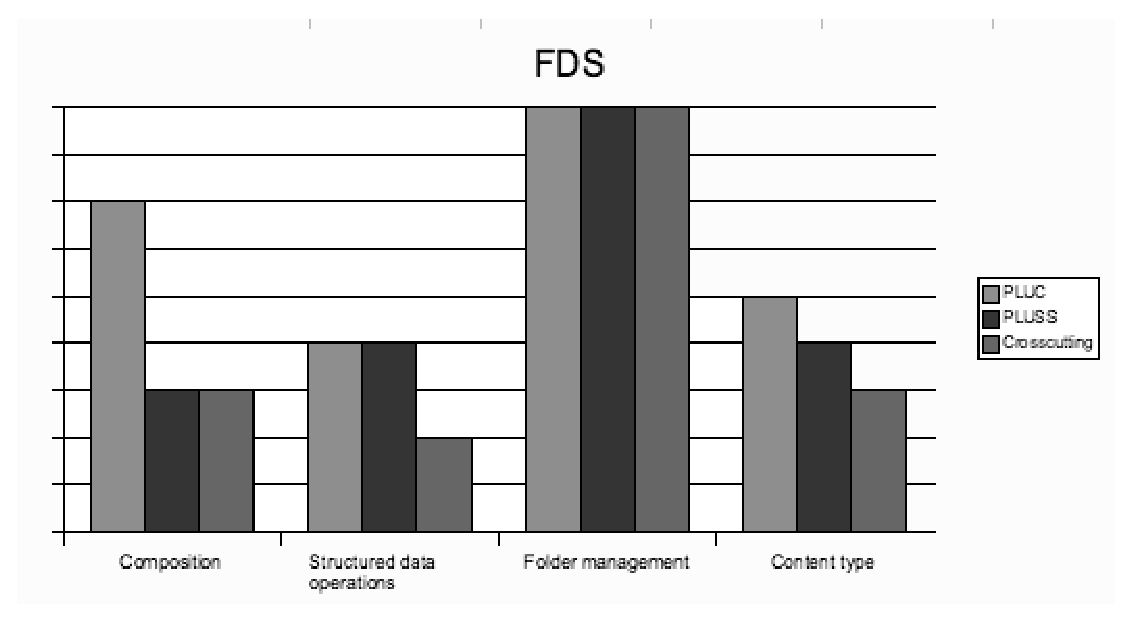
\includegraphics[scale=0.42]{img/fds-mms.eps}
  \nocaptionrule \caption{Relative FDS for evaluated techniques}
  \label{fig:fds-mms}
  \end{center}
\end{figure}

\subsubsection{Pedagogical Product Line}

We compared our approach against two specifications of the Pedagogical Product Line (PPL): the original one~\cite{ppl-url}, proposed by the Software Engineering Institute, and a specification that was sent to us by the authors of the PLUSS technique. 

The original specification of PPL is already well modularized, since its features, in general, are not crosscutting among different use cases (see modularity metrics in Table~\ref{tab:ppl-metrics}). Moreover, another characteristic of PPL is that several features are related to qualities that do not cause effect into use case specifications. 

\begin{table}[hb]
\centering
\nocaptionrule \caption{PPL quantitative evaluation}
\label{tab:ppl-metrics}
\begin{small}
\begin{tabular}{lccc} \hline
					& SEI 	& PLUSS 	& Crosscutting	\\ \hline
Mean value of FDU 		& 1.83	& 1.3	& 1.2	\\
Mean value of FDS 		& 3.3	& 3		& 2.5	\\
Mean value of NFU 		& 2		& 2		& 1.4	\\
Mean value of FSS 		& 3.8	& 3.5	& 3		\\ 
VSU 					& 12		& 7		& 6		\\
VSS 					& 25		& 19		& 16		\\
SS 					& 44		& 38		& 32		\\	\hline
\end{tabular}
\end{small}
\end{table}

Still in this context, our approach also achieves some improvements in the resulting specifications. The main factor for these improvements in the \emph{Pedagogical} product line was the error handling modularization. By applying our approach, all behavior related to the \emph{error handling} concern is specified in a single use case. The composition of \emph{error handling} with the basic scenarios was done by means of annotations attributed to the corresponding steps. For instance, Figure~\ref{fig:error-handle} depicts just one scenario for error handling: raising  an error when there is no space available. 

\begin{figure}[h]
\begin{scriptsize}
  \texttt{
   \begin{tabular}{l}
     Description: There is no available space in file system.\\
     From step: [CatchFileException] \\
     To step: END
   \end{tabular}  
  \begin{center} 
   \begin{tabular}{|p{0.1in}|p{0.6in}|p{1.0in}|p{1.0in}|}
   \hline
       Id & User Action & System State & System Response \\ \hline \hline
       E1 & & There is not enough space to save the file. &  Raise the Disk is Full exception. The arcade game application is finished. \\  \hline
  \end{tabular}
  \end{center}
  } 
\end{scriptsize}
\nocaptionrule \caption{Scenario of error handle use case.}
\label{fig:error-handle}
\end{figure}
    
Notice that this scenario can be started from any step that has been marked with the \emph{CatchFileException} annotation (see the \emph{From step} clause). Several features of the PPL need to save information in the file system. Therefore, both in the SEI and PLUSS specifications of the \emph{Pedagogical} product line, several use cases were specified with scenarios for handling this kind of exception.

As a consequence, we achieve a reduction (almost 20\%) in the number of specification steps (SS in Table~\ref{tab:ppl-metrics}) when comparing to the PLUSS approach. It is important to notice that this reduction of size does not compromise the requirement coverage; but actually it represents an improvement in the specification reuse.

For concluding our Pedagogical product line analysis, we can realize, based on Table~\ref{tab:ppl-metrics}, that our approach achieved real benefits only in the complexity metrics. This result comes from the non crosscutting nature of PPL features. Comparing to the MMS product line results, we argue that the benefits of applying our approach should be greater in contexts where features can not be well modularized using existing techniques. 
   
\section{Related Work}
\label{sec:related}

Our work is linked to the body of research related to SPL
variability management, crosscutting modeling, and use case scenario
composition. This section details some of these approaches, relating
them to the proposed solution.

\subsection{Semantics of Crossuctting Mechanisms}

Masuhara and Kiczales (MK) proposed a modeling framework 
for characterizing implementation techniques as 
\emph{crosscutting mechanisms}~\cite{kiczales-ecoop-2003}. 
A critical property of their model is that two different input 
programs crosscut each other with respect to the resulting 
program or computation. 

In this paper, we applied the MK framework for representing
\emph{variability management} as a crosscutting mechanism. Improving 
modularity is the main reason for representing variability management 
as a crosscutting concern. Actually, we improved both changeability and 
modular reason by applying our approach for managing variabilities 
in use case scenarios(Section~\ref{sec:evaluation}). 

Our proposed framework is used for describing how 
different input SPL specifications crosscut each other to derive 
product specific artifacts. The contribution of each input 
specification is well defined. Observing the whole process, 
not only two specifications are taken as input. Actually, 
in order to derive product specific scenarios, four input 
models are required: feature model, product configuration, 
configuration knowledge, and use case model. Despite that, 
just a few changes were required to applied the MK framework 
in our context. 

\subsection{Variability Management and Feature Modeling}

Pohl et al. argue that variability management should not be
integrated into existing models~\cite{phol-spl-book}. Their proposed
Orthogonal Variability Model (OVM) describes traceability links
between variation points and the conceptual models of a SPL. Our
approach also decouple variability concern. However, we describe, in more
details, its semantics as a crosscutting mechanism. Additionally, we make
clear how to relate SPL features to software engineering assets by means of the
configuration model. In our approach, sucha a model can be used for reasoning 
about traceability.

Feature modeling (FM) has been successfully applied for representing relevant 
characteristics of a SPL, highlighting its common and variant concepts. 
Although different notations for FM have been
proposed~\cite{kang-foda,czarnecki-book,czarnecki-wsfactory-2005}, the 
abstract syntax followed in this paper is based
on~\cite{czarnecki-wsfactory-2005}, supporting constraints,
properties, and cardinality. As a minnor change, in our
work the feature cardinality, described in~\cite{czarnecki-wsfactory-2005}, is
used for identifying the semantics of a feature group (it represents 
an \emph{alternativeFeature} or an \emph{orFeature}). 


\subsection{Scenario Variability}

Several approaches have been proposed for representing 
scenario variability~\cite{jacobson-reuse-book, favaro-icsr-98, eriksson-splc-2005,bertolino-esec-2003}. 
However, in this paper we only compared our crosscutting approach with PLUC and 
PLUSS techniques because they encompass a broad range of SoC between 
variability management and scenario specification. PLUC presents the lowest level of 
modularity, since almost all information related to variability is tangled within use 
cases. Although PLUSS partially reduces such coupling, by considering the 
importance of feature modeling, some dependences from feature to use cases are
still present. These dependences are avoided in our approach.

Design Structure Matrices (DSMs) and crosscutting metrics have being applied 
for assessing modularity in \emph{aspect-oriented} 
systems~\cite{vlopes-aosd-2005,garcia-taosd-2005, greenwood-ecoop-2007}. 
In this work, we also applied DSMs in the context of scenario variability 
management. Moreover, we applied a suite of metrics for quantifying feature 
diffusion and tangling over use cases. Such a suite was first presented
in~\cite{rbonifacio-ea-2008}.


In order to avoid the problem of \emph{fragile point-cuts}, Rashid
et al. proposed a semantic approach for scenario
composition~\cite{rashid-aosd-2007}. Such approach is based on
natural language processing. Using our scenario composition weaver
(Section~\ref{sub:sc-weaver}), a scenario composition can be
represented using references to \emph{step ids} or \emph{step annotations}, 
which also reduce the problem of \emph{fragile point-cut}.

\section{Conclusions}\label{sec:conclusions}

In this paper we formally described variability management as a 
crosscutting mechanism, considering the contribution 
of different input languages that crosscut each other for deriving 
specific members of a product line. 

We applied this notion of variability management in the context of use 
case scenarios, achieving several benefits. First, applying our approach resulted in 
a clear separation of concerns between variability and scenario specifications, 
allowing both representations to evolve independently. Second, we achieved a reduction 
in the size of specifications by composing scenarios in a quantified way. Finally, the 
formal specification allowed us to perform several automatic verification in the composition 
process. This is an interesting characteristic of our approach, since it can be used 
for finding inconsistencies in the final products.

Although our modeling framework was instantiated for representing 
scenario variabilities, we believe that it could be applied in 
other SPL artifacts. Particularly, optional and parameterized artifacts 
are also relevant for non-functional requirements and test cases. 
Additionally, our notion of crosscutting was based on a work that states \emph{what} 
defines a source code technology as supporting crosscutting modularity. Therefore, 
we argue that representing variabilities in source code, using our modeling framework, 
is straightforward.   

%As future work, we would like to apply our notion of variability management in order 
%to identify relationships between
%variabilities at different SPL artifacts (in a first moment, relationships between 
%requirements and test artifacts). Such kind of relationships can help in the product
%generation and traceability activities of a SPL. 
%The modeling
%framework proposed in this work takes a step in this direction, since the 
%composition process used to derive product specific scenarios have been formally represented.

%
% ---- Bibliography ----
%

\bibliographystyle{abbrv}
\bibliography{rbonifacioGPCE}

\end{document}
